%% •••••••••••••••••••••••••••••••••••••••••••••••••••••••••••••••••••••••••••
%% STRUCTURED CUSTOMIZATION OF ARSCLASSICA / CLASSIC THESIS TEMPLATE
%% > so much custom that we ended up dropping both packages, lol...
%% •••••••••••••••••••••••••••••••••••••••••••••••••••••••••••••••••••••••••••



%% ••• GLOBAL BASIC LAYOUT •••••••••••••••••••••••••••••••••••••••••••••••••••
\documentclass[a4,dottedtoc]{scrbook}
\usepackage[top=3cm,bottom=3cm,left=3cm,right=3cm]{geometry} % Custom margins
\usepackage{changepage} % Commands to change the page layout in the middle of 
                        % a document, and to robustly check for typesetting 
                        % on odd or even pages
\usepackage{setspace}   % Needed for \onehalfspacing
\usepackage{calc}       % To perform arithmetic on the arguments of the LATEX 
                        % commands \setcounter,\addtocounter,\setlength, and 
                        % \addtolength [USED SILENTLY!]
%% •••••••••••••••••••••••••••••••••••••••••••••••••••••••••••••••••••••••••••



%% ••• FONTS & ENCODING ••••••••••••••••••••••••••••••••••••••••••••••••••••••
\usepackage[american, italian]{babel} % Multilanguage support: primary=italian
\usepackage[utf8]{inputenc}           % Input encoding: unicode standard UTF-8
\usepackage[T1]{fontenc}              % Output font encoding:  standard 8-bits
\usepackage{amsmath,amssymb,amsthm}   % Mathematical symbols within $<>$ cells
\usepackage{siunitx}                  % International System of Units support
%% •••••••••••••••••••••••••••••••••••••••••••••••••••••••••••••••••••••••••••



%% ••• ARSCLASSICA OVERRIDE ••••••••••••••••••••••••••••••••••••••••••••••••••
%\usepackage[subfig,beramono,eulermath,pdfspacing,listings]{classicthesis}
%\usepackage{arsclassica} % >> SEVERAL PROBLEMS HERE, SEE WARNINGS <<
\renewcommand{\sfdefault}{iwona}
\renewcommand*\sectfont{\sffamily\mdseries\scshape}
\makeatletter
\renewcommand*\l@chapter[2]{%
  \ifnum \c@tocdepth >\m@ne
    \addpenalty{-\@highpenalty}%
    \vskip 1.0em \@plus\p@
    \setlength\@tempdima{1.5em}%
    \begingroup
      \parindent \z@ \rightskip \@pnumwidth
      \parfillskip -\@pnumwidth
      \leavevmode \sffamily\mdseries\scshape
      \advance\leftskip\@tempdima
      \hskip -\leftskip
      #1\nobreak\hfil \nobreak\hb@xt@\@pnumwidth{\hss\normalfont #2}\par
      \penalty\@highpenalty
    \endgroup
  \fi}
\makeatother
%% •••••••••••••••••••••••••••••••••••••••••••••••••••••••••••••••••••••••••••



%% ••• METADATA SETUP ••••••••••••••••••••••••••••••••••••••••••••••••••••••••
%% ••• Information and Commands for Reuse ••••••••••••••••••••••••••••••••••••

\newcommand{\theTitle}
{Valutazione infermieristica della qualità della sedazione procedurale pediatrica}

\newcommand{\theAuthor}
{\protect Ana\"is \textsc{Trinca}}

\newcommand{\theSubject}
{Nursing assessment of the quality of pediatric procedural sedation}

\newcommand{\theKeys}
{sedazione procedurale, pediatria, risveglio, qualità del risveglio}

\newcommand{\theDate}
{Anno Accademico 2021/2022}

\newcommand{\theFirstSupervisor}
{\protect Prof. Egidio \textsc{Barbi}}

\newcommand{\theSecondSupervisor}
{\protect Dott.ssa Martina \textsc{D'Agostin}}

\newcommand{\theCoordinator}
{Roberto Luzzati}

\newcommand{\theUniversity}
{\protect Universit\`a degli Studi di Trieste }

\newcommand{\theDepartment}
{Dipartimento Universitario Clinico di Scienze Mediche, Chirurgiche e della Salute}

\newcommand{\theDegree}
{Corso di Laurea in Medicina e Chirurgia}

\newcommand{\theCity}
{Trieste}

%% ••••••••••••••••••••••••••••••••••••••••••••••••••••••••••••••••••••••••••• % Import defined metadata from a user-accessed friendly file :)
%% •••••••••••••••••••••••••••••••••••••••••••••••••••••••••••••••••••••••••••



%% ••• REFERENCES & BIBLIOGRAPHY •••••••••••••••••••••••••••••••••••••••••••••
\usepackage{varioref} % \vref and \vpageref ('decorated' references...)
\PassOptionsToPackage{
        natbib=true,
        style=ieee,
        dashed=false,           % FIX for IEEE style (same author case)
        citestyle=numeric-comp,
        sorting=nyvt,           % name, year, volume, title
        maxnames=3,
        minnames=1,
        hyperref=true,
        backend=biber,
        parentracker=true,
        url=false,
        doi=false,
        isbn=false,
        eprint=false,
        backref=true,
            } {biblatex}
\usepackage{biblatex}
\stdpunctuation % ANOTHER FIX TO IEEE STYLE
\addbibresource{Bibliografia/Articoli.bib}
\addbibresource{Bibliografia/Testi.bib}
\addbibresource{Bibliografia/Web.bib}
\usepackage[autostyle]{csquotes} % Ensures that quoted texts are typeset 
                                 % according to the rules of the main language 
                                 % > babel required
%% •••••••••••••••••••••••••••••••••••••••••••••••••••••••••••••••••••••••••••



%% ••• GRAPHICAL MAGIC •••••••••••••••••••••••••••••••••••••••••••••••••••••••
\usepackage{subfig}
\usepackage{caption}
\usepackage{graphicx}
\usepackage[x11names]{xcolor}
% THE UNITS OFFICIAL PANTONE [but ugly..]
\definecolor{trieste}{HTML}{29385c} 
% https://usbrandcolors.com/microsoft-colors/
\definecolor{grigiomicrosoft}{HTML}{737373}
\definecolor{rossomicrosoft}{HTML}{F25022}
\definecolor{giallomicrosoft}{HTML}{FFB900}
\definecolor{verdemicrosoft}{HTML}{7FBA00}
\definecolor{blumicrosoft}{HTML}{00A4EF}
% XKCD COLOR-UNIVERSE
\usepackage{xkcdcolors}
% OTHER CUSTOM DEFINED COLORS
\definecolor{grigiochiaro}{RGB}{223,223,222}
\definecolor{teal}{RGB}{65,125,122}
\definecolor{gris}{RGB}{160,188,194}
% FANCY COLORBOXES TO PUT TEXT IN
\newenvironment{fancybox}[1]
{
    \begin{tcolorbox}[
        colback=#1!25,
        colframe=#1!100,
        fonttitle=\sffamily\mdseries\scshape,
        arc=3mm,
        boxrule=0pt]   
}
{
    \end{tcolorbox}
}
%% •••••••••••••••••••••••••••••••••••••••••••••••••••••••••••••••••••••••••••



%% ••• CUSTOM COMMAND-SET FOR QUESTIONNAIRES •••••••••••••••••••••••••••••••••
%%%%%%%%%%%%%%%%%%%%%%%%%%%%%%%%%
%% Required package inclusions %%
%%%%%%%%%%%%%%%%%%%%%%%%%%%%%%%%%

\usepackage{wasysym} % provides $\ocircle$ and $\Box$
\usepackage{forloop} % used for \Qrating and \Qlines
\usepackage[breakable]{tcolorbox} % xcolor required 

%%%%%%%%%%%%%%%%%%%%%%%%%%%%%%%%%%%%%%%%
%% Special colorful boxed environment %%
%%%%%%%%%%%%%%%%%%%%%%%%%%%%%%%%%%%%%%%%
\newenvironment{survey}[2][QUESTIONARIO] 
{
\newcommand{\Qcolor}{#2}
\begin{tcolorbox}
[breakable,
title=#1,
colback=\Qcolor!40,
colframe=\Qcolor!40,
coltitle=black,
colbacktitle=\Qcolor!75,
fonttitle=\sffamily\mdseries\scshape,
halign title=flush center,
arc=3mm,
boxrule=0pt]
\begin{enumerate}
[leftmargin=1.5em,
itemsep=1.5em]
\newcommand{\Query}{\item} % fancy alias
}
{
\end{enumerate}
\end{tcolorbox}
} % USAGE: \begin{survey}[title]{colorname}

%%%%%%%%%%%%%%%%%%%%%%%%%%%%%%%%%%%%%%%%%%%%%%%%%%%%
%% Beginning of questionnaire command definitions %%
%%%%%%%%%%%%%%%%%%%%%%%%%%%%%%%%%%%%%%%%%%%%%%%%%%%%

%% \Qbox -> Empty box to be ticked.
%% > Used both by direct call and by \Qlist itemization.
\fboxsep=1mm \fboxrule=0.6pt
\newcommand{\Qbox}
{\fcolorbox{black}{\Qcolor!10}{\color{\Qcolor!10}$\ocircle$}}
%% > or replace $\ocircle$ with $\Box$, making the resulting box a little wider...

%% \Qlist -> This is an environment very similar to itemize but with
%% \Qbox in front of each list item. Useful for classical multiple
%% choice. Change leftmargin and topsep according to your taste.
\newenvironment{Qlist}{%
\renewcommand{\labelitemi}{\Qbox}
\begin{itemize}[leftmargin=2em]   %[leftmargin=2.57em]%,topsep=-.5em]
}{%                               ^matches itemize    ^no good
\end{itemize}
}

%% \Qnum -> Similar to \Qbox, but it contains a number.
%% > Used within \Qrating.
\newcommand{\Qnum}[1]{\colorbox{\Qcolor!10}{#1}}

%% \Qrating{N} -> Automatically create a rating scale with N steps.
%% > like this: [1] [2] [3] … [N] .
\newcounter{qr}
\newcommand{\Qrating}[1]{\forloop{qr}{0}{\value{qr}<#1}{~\Qnum{\arabic{qr}}}}

%% \Qline -> Again, this is very simple. It helps setting the line thickness globally.
%% > You can change the default width (=\linewidth) with the \Qline{WIDTH} syntax
%% > Used both by direct call and \Qlines newline-iterator.
\newcommand{\Qline}[1]{\noindent\rule{#1}{0.6pt}}

%% \Qlines{N} -> Insert N lines with width=\linewidth (default \Qline). 
%% > You can change the \vskip value to tweak the vertical interspacing.
\newcounter{ql}
\newcommand{\Qlines}[1]{\forloop{ql}{0}{\value{ql}<#1}{\vskip0em\Qline{\linewidth}}}


%% \Qtab -> A "tabulator". The first argument is the distance from the left.
%% The second argument is the content to be indented [no line skip].
\newlength{\qt}
\newcommand{\Qtab}[2]{
\setlength{\qt}{\linewidth}
\addtolength{\qt}{-#1}
\hfill\parbox[t]{\qt}{\raggedright #2}
}

%%%%%%%%%%%%%%%%%%%%%%%%%%%%%%%%%%%%%%%%%%%%%%
%% End of questionnaire command definitions %%
%%%%%%%%%%%%%%%%%%%%%%%%%%%%%%%%%%%%%%%%%%%%%%
%%
%% •••••••••••••••••••••••••••••••••••••••••••
%% COPYRIGHT
%% ···········································
%% © 2010-2012, Sven Hartenstein [original]
%% mail@svenhartenstein.de
%% http://www.svenhartenstein.de
%% ···········································
%% © 2022, G. Bellomia [heavy customization]
%% gabriele.bellomia@sissa.it
%% https://github.com/bellomia
%% •••••••••••••••••••••••••••••••••••••••••••
%%
%% Please be warned that this is NOT a full-featured framework for
%% creating (all sorts of) questionnaires. Rather, it is a small
%% collection of LaTeX commands that I found useful when creating a
%% questionnaire. Feel free to copy and adjust any parts you like.
%% Most probably, you will want to change the commands, so that they
%% fit your taste.
%%%%%%%%%%%%%%%%%%%%%%%%%%%%%%%%%%%%%%%%%%%%%%%%%%%%%%%%%%%%%%%%%%LICENSE % Too long to nicely fit here...
%% •••••••••••••••••••••••••••••••••••••••••••••••••••••••••••••••••••••••••••



%% ••• HYPERLINKS & METADATA •••••••••••••••••••••••••••••••••••••••••••••••••
\usepackage{hyperref}
\hypersetup
{
	%bookmarks=true,            % show bookmarks bar [ALREADY SET BY SCRBOOK]
	unicode=true,               % non-Latin characters in Acrobat’s bookmarks
	pdftoolbar=false,           % show Acrobat’s toolbar?
	pdfmenubar=true,            % show Acrobat’s menu?
	pdffitwindow=false,         % window fit to page when opened
	pdfstartview={FitH},        % fits the width of the page to the window
	pdfauthor={\theAuthor},     % digital author in the PDF metadata
	pdftitle={\theTitle},       % digital title in the PDF metadata
	pdfsubject={\theSubject},   % digital subject in the PDF metadata
	pdfkeywords={\theKeys},     % digital keywords in the PDF metadata
	pdfcreator={Overleaf},      % platform generating the PDF source
	pdfproducer={PdfLaTeX},     % app producing the PDF build
	pdfnewwindow=true,          % links in new PDF window
	colorlinks=true,            % false: boxed links; true: colored links
	linkcolor=trieste,          % color of internal links
	citecolor=trieste,          % color of links to bibliography
	filecolor=trieste,          % color of file links
	 urlcolor=trieste           % color of external links
}
%% •••••••••••••••••••••••••••••••••••••••••••••••••••••••••••••••••••••••••••



%% ••• APPENDIX SETUP ••••••••••••••••••••••••••••••••••••••••••••••••••••••••
\usepackage[toc,page]{appendix}
\renewcommand{\appendixname}{Appendici}
\renewcommand{\appendixtocname}{Appendici}
\renewcommand{\appendixpagename}{\sffamily\mdseries\scshape Appendici}
%% •••••••••••••••••••••••••••••••••••••••••••••••••••••••••••••••••••••••••••



%% ••• LISTINGS SETUP ••••••••••••••••••••••••••••••••••••••••••••••••••••••••
\usepackage{listings}          % Monospaced environments, highly customizable
\usepackage{matlab-prettifier} % Special wrapper of listings, aimed at mfiles
\lstset{
    style=Matlab-editor,
    basicstyle=\mlttfamily\small,
	backgroundcolor=\color{grigiomicrosoft!0}, 
	mlsectiontitlestyle=\bfseries\color{verdemicrosoft},
	mlcommentstyle=\color{giallomicrosoft},
	numberstyle=\mlttfamily\color{grigiomicrosoft!50},
	mlstringstyle=\color{rossomicrosoft},
	mlkeywordstyle=\color{blumicrosoft},
	mlsharedvars={ palette,
	               boxplot,
                   hex2rgb,
                   matverse,
				   fig2svg,
				   save_fig,
	               export_fig,
	               kruskalwallis,
	               multcompare,
	               },
	mlsharedvarstyle=\bfseries\itshape\color{xkcdLilac},
	breakatwhitespace=true,         
	breaklines=true,                 
	captionpos=b,                    
	keepspaces=true,                 
	numbers=left,                    
	numbersep=5pt,                  
	showspaces=false,                
	showstringspaces=true,
	showtabs=true,                  
	tabsize=4,
	xleftmargin=25pt,
    }
\lstset{
    literate=%
    {æ}{{\ae}}1
    {å}{{\aa}}1
    {ø}{{\o}}1
    {Æ}{{\AE}}1
    {Å}{{\AA}}1
    {Ø}{{\O}}1
    {à}{{\`a}}1
    {è}{{\`e}}1
    {ì}{{\`i}}1
    {ò}{{\`o}}1
    {ù}{{\`u}}1
    {á}{{\'a}}1
    {é}{{\'e}}1
    {í}{{\'i}}1
    {ó}{{\'o}}1
    {ú}{{\'u}}1
    {ã}{{\~a}}1
    {õ}{{\~o}}1
    {â}{{\^a}}1
    {ê}{{\^e}}1
    {î}{{\^i}}1
    {ô}{{\^o}}1
    {û}{{\^u}}1
    {È}{{\`E}}1
    {Š}{{\v{S}}}1
    {°}{{\degree}}1
    }
%% •••••••••••••••••••••••••••••••••••••••••••••••••••••••••••••••••••••••••••



%% ••• OTHER STUFF •••••••••••••••••••••••••••••••••••••••••••••••••••••••••••
\usepackage{multicol}                % Multicolumn environment, made easy
\usepackage{makeidx}                 % Standard package for creating indexes
\usepackage{relsize}                 % \larger, \smaller, \textlarger, etc.
\usepackage{lipsum}                  % Lorem Ipsum text-fillers
\usepackage{epigraph}                % Quotes, jokes, riddles... made nice
\usepackage{comment}                 % Silencing huge parts of source code
\usepackage{tablefootnote}           % Footnotes inside table environments
\usepackage[shortlabels]{enumitem}   % Enumerate with letters
\setlist[description]{               % Enumerate with full captions
  %topsep=30pt,                      % > space before start/after end of list
  %itemsep=5pt,                      % > space between items
  font={\sffamily\mdseries\scshape}, % > set the label font
}
%% •••••••••••••••••••••••••••••••••••••••••••••••••••••••••••••••••••••••••••






%%%%%%%%%%%%%%%%%%%%%%%%%%%%%%%%%%%%%%%%%%%%%%%%%%%%%%%%%%%%%%%%%%%%%%%%%%%%%%
%%%%%%%%%%%% ···················································· %%%%%%%%%%%%
%%%%%%%% ···························································· %%%%%%%%
%%%%% ·································································· %%%%%
%%% ······································································ %%%
%% •••••••••••••••••••••••••••••••••••••••••••••••••••••••••••••••••••••••• %%
% >> NON METTERE MANO A NULLA SOPRA QUESTA FASCIA (SE NON AUTORIZZATI) :P << %
%% •••••••••••••••••••••••••••••••••••••••••••••••••••••••••••••••••••••••• %%
%%% ······································································ %%%
%%%%% ·································································· %%%%%
%%%%%%%% ···························································· %%%%%%%%
%%%%%%%%%%%% ···················································· %%%%%%%%%%%%
%%%%%%%%%%%%%%%%%%%%%%%%%%%%%%%%%%%%%%%%%%%%%%%%%%%%%%%%%%%%%%%%%%%%%%%%%%%%%%






%% ••• DARK-THEME SWITCH •••••••••••••••••••••••••••••••••••••••••••••••••••••
%\pagecolor[RGB]{40,42,54} % Dracula-theme: background
%\color[RGB]{248,248,242}  % Dracula-theme: foreground
%% •••••••••••••••••••••••••••••••••••••••••••••••••••••••••••••••••••••••••••






\begin{document}

%>FRONTESPIZIO
\newgeometry{top=0cm,bottom=1cm,left=3cm,right=3cm}
%----------------------------------------------------------------------------------------
%	TITLE PAGE
%----------------------------------------------------------------------------------------

\begin{titlepage} % Suppresses displaying the page number on the title page and the subsequent page counts as page 1
\pdfbookmark{Titlepage}{Titlepage}
\changetext{}{}{}{((\paperwidth  - \textwidth) / 2) - \oddsidemargin - \hoffset - 1in}{}
\null\vfill
\begin{center}
\large
\sffamily
	\newcommand{\HRule}{\rule{\linewidth}{0.5mm}} % Defines a new command for horizontal lines, change thickness here
	
	\center % Centre everything on the page
	
	%------------------------------------------------
	%	Logo
	%------------------------------------------------
	
	%\vfill
	\includegraphics[width=0.3\textwidth]{Figure/logoUniTs_tondo.pdf}\\[1cm] % Include a department/university logo - this will require the graphicx package
	 
	%----------------------------------------------------------------------------------------
	
	%------------------------------------------------
	%	Headings
	%------------------------------------------------
	
	\textsc{\LARGE Universit\`a degli Studi di Trieste}\\
	\HRule\\[0.5cm] % Main heading such as the name of your university/college
	
	\textsc{\Large Dipartimento Universitario Clinico di Scienze Mediche, Chirurgiche e della Salute}\\[0.5cm] % Major heading such as course name
	
	\textsc{\large Corso di Studi in Medicina e Chirurgia}\\[0.5cm] % Minor heading such as course title
	
	%------------------------------------------------
	%	Title
	%------------------------------------------------
	
	\vfill
	
	{\huge\bfseries Un Titolo Monello}\\[0.2cm] % Title of your document
	
	\vfill
	
	%------------------------------------------------
	%	Author(s)
	%------------------------------------------------
	
	\begin{minipage}{0.4\textwidth}
		\begin{flushleft}
			\large
			\textit{Candidata}\\
			Ana\"is \textsc{Trinca}\\ % Your name
			\small{ME0300935}
		\end{flushleft}
	\end{minipage}
	~
	\begin{minipage}{0.4\textwidth}
		\begin{flushright}
			\large
			\textit{Relatore}\\
			dott. Gianni \textsc{Biolo} % Supervisor's name
		\end{flushright}
	\end{minipage}
	
	% If you don't want a supervisor, uncomment the two lines below and comment the code above
	%{\large\textit{Author}}\\
	%John \textsc{Smith} % Your name
	
	%------------------------------------------------
	%	Date
	%------------------------------------------------
	
	\vfill\vfill\vfill % Position the date 3/4 down the remaining page
	
	{\large \textsc{Anno Accademico 2019/2020}} % Date, change the \today to a set date if you want to be precise
	
	\vfill % Push the date up 1/4 of the remaining page
	\end{center}
\end{titlepage}

%----------------------------------------------------------------------------------------
\frontmatter
\restoregeometry
\null\vfill
\begin{flushright}
{\ttfamily } \emph{Dedica bla bla bla}
\end{flushright}
\vfill\vfill

%>INDICE[AUTOMATIZZATO]
\tableofcontents

%>GLOBAL-SETUP
\mainmatter
\onehalfspacing % layout "arieggiato"

%>CAPITOLI
\chapter{Introduzione}

\section{A section}

\lipsum[1]

\subsection{A subsection}

\lipsum[2]

\subsubsection{A subsubsection}

\lipsum[3]
\chapter{Materiali e Metodi}
%\`E

Questo lavoro di tesi è basato su uno studio osservazionale prospettico condotto presso l'ospedale universitario di terzo livello, istituto materno infantile --- IRCSS Burlo Garofolo di Trieste. In tale analisi si esamina il livello di soddisfazione percepito dal personale infermieristico in merito alla qualità della sedazione pediatrica al di fuori della sala operatoria, mettendo a confronto quattro agenti sedativi ed analgesici tra i più ampiamente utilizzati: propofol, midazolam, ketamina e dexmedetomidina. 
\\Dal momento che in letteratura non esiste uno strumento validato per la valutazione della percezione infermieristica, è stato formulato da un gruppo di pediatri, anestesisti pediatrici ed infermieri pediatrici un questionario appositamente designato agli scopi di questo studio. Dopo essere stato testato su un campione ridotto di 30 soggetti ed essere stato rifinito e corretto sulla base delle raccomandazioni fornite da questi primi partecipanti, è stato infine sottoposto a 51 infermieri esperti nel campo della sedazione peri-procedurale.

\section{Scelta dell'infermiere come indicatore di qualità}

La scelta di valutare la percezione del personale infermieristico deriva dalla necessità di ampliare ed oggettivare i risultati emersi nello studio riguardante la soddisfazione parentale, ampiamente descritto poco sopra \cite{Cortellazzo2022}. Infatti, mentre il caregiver viene facilmente influenzato da diversi fattori associati alla totalità del vissuto ospedaliero, dal servizio di parcheggio, alla simpatia del personale, finanche alla comparsa di complicanze correlate specificamente alla procedura; l'infermiere assiste mensilmente innumerevoli pazienti durante tutte le fasi della procedura: dall'ammissione, al posizionamento dell'accesso venoso, al monitoraggio dei parametri vitali e alla somministrazione dei farmaci prima e durante la sedazione, fino poi al completo risveglio ed alla dimissione. Risulta quindi il candidato più adatto a giudicare in maniera oggettiva gli elementi associati alla sedazione ed al risveglio post procedurale. Inoltre, mentre il genitore esprime il proprio parere basandosi su un'unica o su limitate esperienze di analgosedazione, l'infermiere partecipa a molteplici sedazioni procedurali ogni mese ed è quindi in grado di confrontare diversi regimi farmacologici ed esprimere un giudizio qualitativo basato sull'efficacia della sedazione, sulla facilità e sulla sicurezza della via di somministrazione, oltre che sull'incidenza e la severità degli effetti avversi associati.
\\In conclusione, l'opinione dell'infermiere riveste un ruolo chiave non solo al fine di ottenere delle indicazioni utili per la scelta farmacologica ma anche come occasione per integrare le conoscenze mediche alle osservazioni di una figura di riferimento fondamentale per il paziente e la famiglia, quale quella dell'infermiere. La collaborazione tra la professionalità medica ed infermieristica rappresenta il presupposto migliore per garantire alla comunità una sempre maggiore attenzione alla qualità di cura. 



%in maniera risulta un candidato più adatto a giudicare in modo oggettivo  Inoltre, 



%Dalle conclusioni dello studio sopra descritto sulla soddisfazione parentale in merito alla sedazione procedurale pediatrica \cite{Cortellazzo2022}, è emersa la necessità di estendere l'analisi ad una figura professionale che possa confrontare fornire un giudizio oggettivo. Infatti, il caregiver può essere influenzato nella valutazione finale dall'esperienza medico ospedaliera vissuta nella sua interezza, che può includere alcune variabili non strettamente associate alla sedazione in sé, quali ad esempio la facilità di parcheggiare, la simpatia del personale, il coinvolgimento nel processo decisionale ed eventuali problematiche specificamente collegate alla procedura. Inoltre, esprime la propria opinione sulla base, nella maggior parte dei casi, di un'unica o di limitate esperienze di analgosedazione e possiede, quindi, scarse o nulle conoscenze rispetto ai regimi farmacologici alternativi. 
%La scelta dell'infermiere come indicatore di qualità della sedazione procedurale ha il compito sia di rispondere all'esigenza di ottenere dei risultati basati su un giudizio più oggettivo, sia di rappresentare un'opportunità di migliorare lo standard di cure e la qualità del risveglio post sedazione. Gli infermieri arruolati in questo lavoro di tesi sono tutti professionisti esperti nel campo della sedazione peri-procedurale, prendono parte mensilmente ad un numero variabile di procedure attuate con regimi farmacologici differenti, assistendo il paziente nelle fasi che precedono e seguono la procedura, fino al completo risveglio ed alla dimissione; inoltre posizionano i cateteri venosi periferici e cooperano con il medico durante la sedazione somministrando i farmaci e monitorando i parametri vitali del bambino. Concludendo, l'infermiere risulta il candidato più adatto a comparare i diversi regimi sedativi e può rappresentare la chiave di volta nel fornire delle indicazioni imparziali, che possano essere utili al sedatore per la scelta farmacologica. Inoltre, questa analisi pone le basi per un potenziare la collaborazione tra medico ed infermiere e garantire al paziente ed alla famiglia una sempre maggiore attenzione alla qualità di cura.

%al fine di migliorare lo standard di cure e la qualità del risveglio post sedazione
%A tale proposito l'infermiere potrebbe essere il candidato più adatto,
%circa la scelta del genitore come indicatore di qualità del servizio sanitario offerto in merito alla sedazione procedurale,
%, invece, potrebbe rispondere all'esigenza di oggettivare la percezione 
%che, comprendendo il giudizio infermieristico, permette di approfondire il rapporto medico-infermiere,

%l'analisi della sua percezione
\section{Questionario}


\section{Analisi Statistica}

%\lipsum[2]
\chapter{Risultati}

\begin{figure}[h]
    \centering
    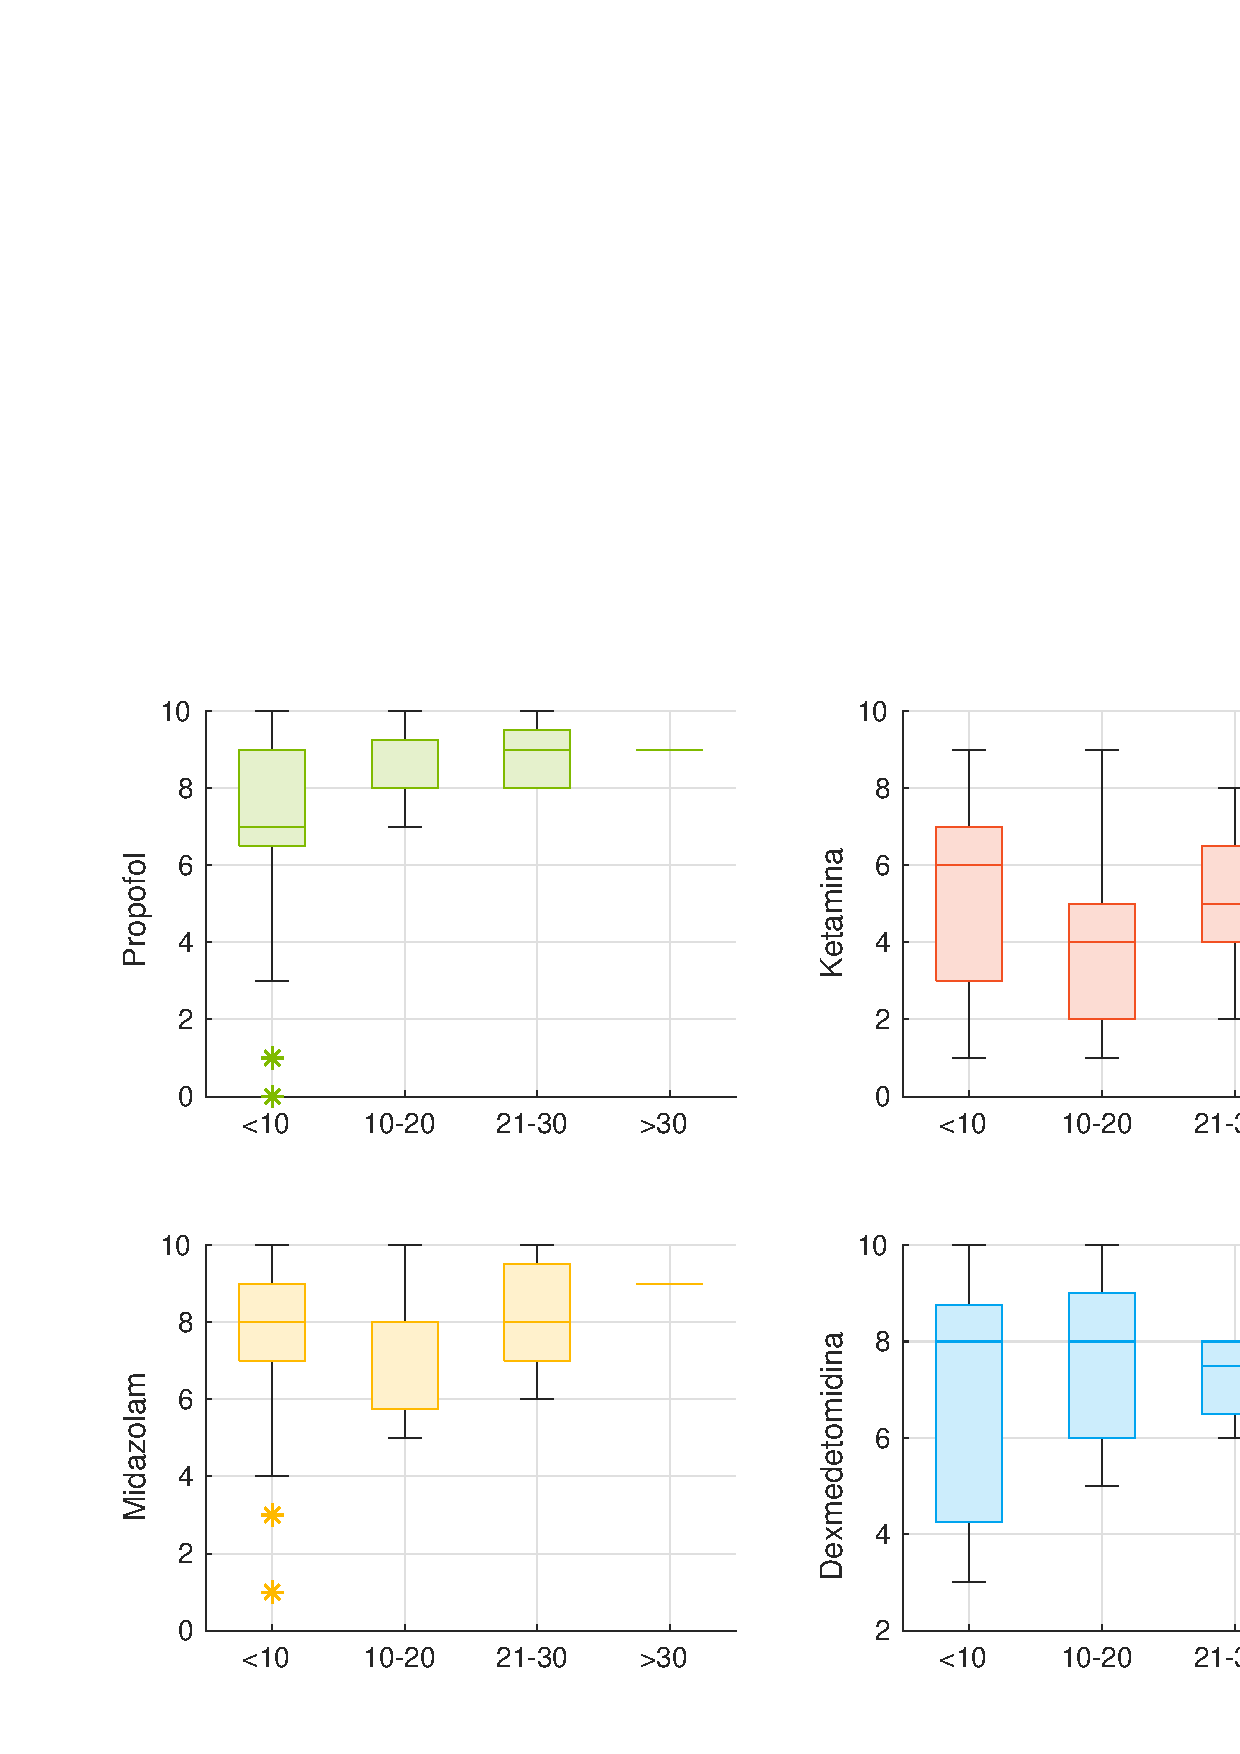
\includegraphics[width=0.8\textwidth]{Figure/qualita-stratificata.pdf}
    \caption{Livello di soddisfazione associato ai diversi agenti farmacologici (misurato secondo scala NRS) stratificato per il numero di sedazioni mensilmente assistite dagli intervistati.}
    \label{fig:qualitastratificata}
\end{figure}
\chapter{Discussione}
%\`E

Questo lavoro si basa sulla convinzione che l'opinione infermieristica sia un indicatore fondamentale per valutare la qualità del servizio di cura offerto quotidianamente ai pazienti pediatrici che si sottopongono a procedure diagnostiche o terapeutiche. Da questo presupposto nasce la volontà di studiare e confrontare le considerazioni e le critiche di una categoria professionale che, oltre ad essere parte attiva durante tutto il percorso di sedazione, spesso riconosce e risponde per prima ai bisogni fisici e psicologici dei piccoli pazienti. Le prospettive di quest'area di ricerca, tutt'ora poco esplorata, stanno nella possibilità di implementare nella pratica medica quotidiana i risultati emersi, agendo sia, laddove possibile, sulla scelta farmacologica, sia sulla comunicazione ed il potenziamento del lavoro di squadra tra medici ed infermieri, garantendo ai pazienti e alle famiglie un'assistenza sempre di maggior qualità e successo. 



%In particolare, in questo studio, lo scopo del raccogliere le opinioni degli infermieri risiede nella volontà di analizzare le considerazioni e le critiche di una categoria professionale che, oltre ad essere parte attiva durante tutto il percorso di sedazione, spesso riconosce e risponde per prima ai bisogni fisici e psicologici dei piccoli pazienti. L'interesse in quest'area di ricerca, tutt'ora poco esplorata, sta nella possibilità di implementare nella pratica medica quotidiana i risultati emersi, agendo sia, laddove possibile, sulla scelta farmacologica, sia sulla comunicazione ed il potenziamento del lavoro di squadra tra medici ed infermieri, garantendo ai pazienti e alle famiglie un'assistenza sempre di maggior qualità e successo. 
\section{Preferenze farmacologiche ed effetti avversi}

\subsection*{Il propofol è stato il farmaco più apprezzato}
Dalla presente analisi emerge che circa metà degli infermieri intervistati preferisce il propofol agli altri agenti farmacologici testati per le sedazioni procedurali. Questo dato risulta in linea con alcuni studi, in cui il propofol, comparato ad altri regimi farmacologici, si rivela un agente altrettanto efficace ma con dei tempi di recupero più brevi e delle caratteristiche di risveglio più favorevoli \citep{Schacherer2019, Havel1999, Shah2011}. Inoltre, il punteggio di soddisfazione associato al propofol aumenta con il numero di sedazioni mensilmente effettuate.

\subsection*{La ketamina ha ottenuto i valori di soddisfazione più bassi}
Il livello di soddisfazione complessivo percepito dai partecipanti si è delineato ugualmente elevato per il propofol, per il midazolam e per la dexmedetomidina, mentre è risultato significativamente inferiore per la ketamina. Gli elementi che hanno influito di più su questo giudizio sono stati la qualità del risveglio e gli effetti avversi: i più frequentemente riportati dagli infermieri sono gli stessi già ampiamente conosciuti in letteratura \citep{Bellolio2016, Krauss2006}. Tra questi il distress respiratorio, le allucinazioni, la nausea e il vomito, le vertigini, l'irritabilità e l'iperattività sono gli effetti collaterali che hanno avuto una maggior influenza sul punteggio complessivo della qualità della sedazione. Alla luce di ciò, è interessante notare come la nausea e il vomito, le allucinazioni, l'irritabilità e l'iperattività coincidano con le reazioni avverse più frequentemente indicate dagli infermieri relativamente alla sedazione con la ketamina\footnote{Il distress respiratorio non è stato riscontrato dagli infermieri per nessuno dei quattro agenti farmacologici testati.}. Inoltre, essa è stata associata anche ad una maggior necessità di farmaci \emph{rescue} o sintomatici, ad esempio antiemetici.
Nonostante la ketamina sia considerata gold standard dai pediatri per la sua efficacia e l'elevata sicurezza \citep{Krauss2006}, l'opinione degli infermieri mette in evidenza alcuni limiti, per lo più relativi alle caratteristiche del risveglio. Un'alternativa possibile è rappresentata dal propofol, il quale possiede un sovrapponibile profilo di sicurezza ed efficacia per quanto concerne le sedazioni procedurali minimamente e moderatamente dolorose \citep{Vardi2002, Ferguson2016, Jalili2016}; inoltre, è stato correlato principalmente a sonnolenza, un effetto avverso di minor impatto sulla percezione infermieristica. In conclusione, quest'indagine conferma l'importanza di una valutazione che tenga conto delle opinioni dei professionisti di tutta l'équipe, al fine di definire le strategie farmacologiche migliori per ogni paziente.

\section{Livello di sicurezza percepito per i quattro agenti farmacologici}
Gli intervistati hanno riferito di sentirsi molto sicuri durante le sedazioni con tutti e quattro gli agenti farmacologici, nonostante queste non siano prive di rischi \citep{Bellolio2016}. Questo risultato dovrebbe incoraggiare l'uso sistematico di sedativi ed analgesici nei bambini che devono sottoporsi a procedure diagnostiche o terapeutiche, purché la sedazione avvenga in setting adeguati, con personale appropriatamente formato e sotto un attento monitoraggio. 

\subsection*{Midazolam vs dexmedetomidina}
Il midazolam è stato indicato dagli infermieri come farmaco più sicuro rispetto alla dexmedetomidina. Nonostante il valore di significatività statistica di tale risultato sia molto vicino ad $\alpha$ (p--value 0.048) e quindi poco rilevante dal punto di vista statistico, ci sono alcune ragioni che potrebbero sottostare a questa risposta. Nel centro in cui è stato svolto questo lavoro di tesi, il midazolam viene utilizzato prevalentemente a dosaggi bassi, al fine di ottenere il solo effetto ansiolitico: ad esempio, per ridurre l'ansia preprocedurale e facilitare il posizionamento dell'accesso venoso periferico. Il rischio di depressione respiratoria associato alla somministrazione del midazolam è dose correlato e, quindi, limitato con tale posologia, inoltre eventuali reazioni avverse possono essere rapidamente annullate grazie al flumazenil, un antagonista delle benzodiazepine. La dexmedetomidina, invece, è indubbiamente un farmaco con un elevato profilo di sicurezza \citep{Sulton2016} e per tale ragione, oltre che per il livello di efficacia, è stato considerato da alcuni studi superiore al midazolam \citep{Barends2017, Lin}. Tuttavia, andando ad analizzare il livello di soddisfazione dei familiari rispetto alla sedazione con questo farmaco si possono fare alcune considerazioni. La dexmedetomidina viene frequentemente utilizzata nei pazienti più piccoli per studi radiologici lunghi, quali la RM. L'ambiente ristretto in cui si svolge tale esame, in un lavoro, ha influenzato negativamente il grado di soddisfazione parentale \citep{Lew2010}. Inoltre, può presentare tempi di recupero più lunghi di altri agenti farmacologici: questo elemento, il tipo di procedura e l'età più bassa dei bambini sottoposti a questo tipo di sedazione ha portato, secondo gli autori di un altro studio \citep{Cortellazzo2022}, la combinazione dexmedetomidina + midazolam, ad ottenere, dai genitori, dei punteggi di soddisfazione inferiori rispetto agli altri regimi farmacologici, seppur complessivamente elevati.


%sulla soddisfazione del caregiver, riportato estesamente nella sezione 1.1., come possibili fattori determinanti il punteggio relativ  pediatriche questi motivi la combinazione di dexmedetomidina e midazolam ha ricevuto i voti più bassi anche nello studio relativo alla soddisfazione parentale in merito alle sedazioni procedurali pediatriche \citep{Cortellazzo2022}, riportato nella sezione 1.1.  

%La ketamina è considerato un gold standard dai pediatri a causa della sua efficacia e sicurezza. Tuttavia, nel contesto delle sedazioni procedurali da minimamente a moderatamente dolorose il propofol potrebbe essere altrettanto efficace e sicuro. Quest'evidenza suggerisce che l'opinione degli infermieri dovrebbe essere condivisa/appoggiata/sostenuta nell'ambito di un lavoro di squadra nel definire una strategia di sedazione per specifico paziente. La soddisfazione infermieristica per il propofol aumenta con il numero di sedazioni eseguite per mese. 

\section{Vie di somministrazione preferite e tecniche di distrazione}
Le vie di somministrazione preferite dal personale infermieristico sono risultate la via endovenosa e la via intranasale più la via orale. Oltre a ciò, il 74.5$\%$ degli infermieri ha giudicato le tecniche di distrazione come importanti o molto importanti. Quest'ultime sono semplici, economiche, facili da imparare e non richiedono tempi di applicazione eccessivi. Precedenti studi hanno dimostrato l'efficacia dell'approccio non farmacologico, da solo o in combinazione al trattamento farmacologico \citep{Tibaldo2020, Koller2012}: permette, infatti, di controllare il dolore associato a interventi minimamente dolorosi, come le punture venose, di distogliere l'attenzione del bambino dalla procedura, di ridurre la paura e, quindi, di favorire la collaborazione. La consapevolezza degli infermieri in merito alla rilevanza delle tecniche di distrazione rappresenta per tutti i medici un solido promemoria dell'importanza di questa centrale componente della cura. 
%La via EV e la IN + OS sono le preferite da questa ricerca. Il 74.5 degli intervistati ha votato le tecniche di distrazione come importanti. Infatti, sono semplice, economiche, facili da imparare, non dispendiose in termini di tempo. Precedenti studi hanno visto che gli interventi non farmacologici nei pazienti pediatrici riducono il dolore associato a procedure minimamente dolorose quali venipunture, e hanno mostrato che queste tecniche, da sole o in combinazione con il trattamento farmacologico possono ridurre il dolore e la paura, oltre a promuovere la collaborazione di bambino e genitori. La consapevolezza degli infermieri rispetto alla rilevanza delle tecniche non farmacologiche e un adeguata comunicazione con pazienti e famiglie è un forte promemoria per tutti i medici dell'importanza di questa determinante/cruciale/centrale/decisivo componente di cura. 

%Indipendentemente dal regime farmacologico, hanno riportato di sentirsi sicuri durante le sedazioni procedurali anche se non sono completamente prive di rischio (cit). Questo risultato dovrebbe incoraggiare l'uso sistematico dei sedativi nei setting adeguati con definiti livelli di training e monitoraggio per i bambini che si sottopongono a procedure diagnostiche o terapeutiche che causano dolore o stress eccessivo. Gli eventi avversi più frequentemente riportati sono quelli già conosciuti in letteratura (cit.) Distress respiratorio, allucinazioni e nausea/vomito hanno avuto un impatto maggiore. 

\section{Limiti dello studio}
Questo lavoro ha alcune limitazioni. Innanzitutto, è stato utilizzato un questionario non validato, dal momento che non è disponibile in letteratura uno strumento validato per raccogliere i dati necessari agli scopi di questa ricerca. Secondariamente, il numero di infermieri intervistati è relativamente ridotto poiché l'indagine è stata limitata ad un singolo centro. Inoltre, molti infermieri potrebbero non aver avuto esperienza con tutti i tipi di sedativi ed analgesici testati. 

\section{Punti di forza dello studio}
I punti di forza di quest'analisi consistono sia nell'arruolamento di infermieri pediatrici con rilevante esperienza nel campo delle sedazioni procedurali, sia nella realizzazione in due tempi del questionario, la cui versione definitiva è frutto del contributo congiunto di medici, infermieri e genitori. 
\chapter{Conclusioni}

Questo studio ha mostrato che, tra i farmaci più comunemente utilizzati per la sedazione pediatrica al di fuori della sala operatoria, il propofol, il midazolam e la dexmedetomidina sono i più apprezzati dagli infermieri. Diversamente, la ketamina è stata associata a livelli di soddisfazione significativamente inferiori. Ad ogni modo, la sicurezza percepita durante la sedazione dagli intervistati è risultata elevata per tutti i regimi farmacologici testati. Ad incidere maggiormente sul giudizio degli infermieri sono stati i principali effetti collaterali riscontrati durante e dopo la procedura e la qualità generale del risveglio. 
In ultima analisi, questo studio ha messo in luce la rilevanza dell'opinione infermieristica nell'ambito delle sedazioni procedurali pediatriche, con l'auspicio che una prospettiva multi-professionale possa, in generale, essere presa in considerazione anche in altri campi, al fine di favorire la cooperazione tra professionisti e migliorare la qualità del servizio offerto. 

%>APPENDICI
\begin{appendices}
\chapter{La sedazione procedurale}

La sedazione procedurale è una pratica sempre più diffusa ed utilizzata in una moltitudine di setting in tutto il mondo, anche da professionisti senza una formazione anestesiologica specifica. In ambito pediatrico, considerata l'importanza di offrire analgesia ed ansiolisi, tenendo conto anche delle tappe dello sviluppo psicofisico del bambino e al fine di prevenire la memoria di un vissuto negativo, viene quotidianamente eseguita per un vasto numero di procedure, sia in elezione che in urgenza. 

\section{Definizione}

La sedazione è uno stato di depressione della coscienza, con contestuale riduzione di vigilanza e consapevolezza, indotto dall'utilizzo di farmaci sedativi, ipnotici e dissociativi\footnote{I farmaci più comunemente utilizzati sono riportati nell'appendice B.} con o senza proprietà analgesiche. Questa condizione progredisce, senza una divisione arbitraria, lungo un \emph{continuum}: da un grado di sedazione minimo (o ansiolisi) ad un livello ben più profondo di anestesia generale, che richiede il supporto anestesiologico, attraversando le tappe della sedazione moderata e profonda \cite{Krauss2006}. \`E compito del sedatore conoscere le proprietà dei farmaci utilizzati e titolarli adeguatamente al fine di ottenere il livello di sedazione anticipatamente designato.  
\\Si definisce \emph{procedurale} quando viene attuata al di fuori del teatro operatorio per lo svolgimento di procedure diagnostiche e/o terapeutiche di breve durata, con il raggiungimento di un grado massimo di sedazione profonda e quindi con il mantenimento della funzionalità cardiorespiratoria e dei riflessi protettivi delle vie aeree. 

Nonostante non esista un preciso confine tra un livello di sedazione ed il successivo, i principali stati di depressione della coscienza ottenibili possono essere descritti come segue~\cite{Statpearls, Berkenbosch2015}:

\begin{description}
\item[Analgesia] Trattamento del dolore senza alterazione intenzionale dello stato mentale.
\item[Sedazione minima] Anche detta ansiolisi; il paziente è sveglio e risponde normalmente allo stimolo verbale. Le funzioni cognitive e di coordinazione potrebbero essere minimamente alterate, mentre la funzionalità cardiorespiratoria non è influenzata.
\item[Sedazione moderata] Il paziente ha un livello di coscienza depresso ma risponde allo stimolo verbale, eventualmente accompagnato da una leggera sollecitazione tattile. Le vie aeree vengono mantenute pervie senza necessità di intervento e la funzionalità cardiorespiratoria è inalterata. 
\item[Sedazione profonda] Il paziente risulta difficilmente risvegliabile ma potrebbe rispondere a ripetuti stimoli verbali o dolorosi. Inoltre, potrebbe necessitare di supporto per mantenere le vie aeree pervie mentre la funzionalità cardiorespiratoria è solitamente inalterata. 
\item[Anestesia generale] Il paziente non è risvegliabile e necessita di supporto per mantenere le vie aeree pervie ed una ventilazione adeguata, infatti si accompagna solitamente a depressione respiratoria e cardiovascolare. 
\item[Sedazione dissociativa] La sedazione con ketamina rappresenta un'eccezione al continuum tra i diversi livelli di sedazione su cui si muovono gli altri agenti farmacologici. Infatti, i suoi effetti terapeutici sono correlati a specifici dosaggi, rappresentati nella tabella~\ref{tab:1}. Dal punto di vista sedativo, porta il paziente in uno stato catalettico, simile alla trance, in cui il paziente è insensibile agli eventi esterni e sperimenta profonda analgesia ed amnesia, tuttavia rimane sveglio e mantiene intatti la respirazione, i riflessi protettivi e la stabilità cardiopolmonare.

\end{description}

\section{Gli scopi}

I principali obiettivi per cui si effettuano le sedazioni procedurali sono \cite{Uptodatesed}: 

\begin{itemize}
    \item Garantire il benessere e l'incolumità del paziente durante tutte le fasi della procedura.
    \item Trattare l'ansia, indurre amnesia ed evitare un possibile trauma psicologico associato ad un'esperienza spiacevole e di difficile comprensione per il paziente pediatrico.
    \item Ridurre al minimo la percezione del dolore ed evitare un'eventuale risposta vagale alla procedura dolorosa.
    \item Limitare il movimento al fine di permettere una riuscita della procedura sicura ed efficace.

\end{itemize}

Questi scopi possono essere raggiunti al meglio utilizzando il farmaco al dosaggio più basso possibile che contestualmente consenta di ottenere l'effetto terapeutico desiderato \cite{Guidelines2019}.

\section{La formazione del sedatore}

Soprattutto in ambito pediatrico, per i motivi precedentemente esposti, c'è un ampia e crescente richiesta di figure qualificate, che possiedano le competenze adeguate a svolgere in sicurezza e con efficacia le sedazioni procedurali. Tale ruolo, storicamente di pertinenza dell'anestesista, viene sempre più praticato in tutto il mondo da una moltitudine di professionalità diverse. Da qui nasce l'esigenza di formare al meglio il personale incaricato dello svolgimento di tali sedazioni; nonostante non esistano ancora delle linee guida internazionalmente condivise sulle abilità di base che dovrebbe possedere un sedatore, ci sono due competenze chiave con cui tale professionista deve avere certamente destrezza: la gestione delle vie aeree e la rianimazione cardiopolmonare con supporto di defibrillatore. Parallelamente, un altro punto fondamentale che deve essere soddisfatto prima di procedere con la sedazione, riguarda la designazione di un team di emergenza, pronto ad intervenire in caso di complicanze che richiedano un livello di cure più avanzato.
\\Oltre a ciò ci sono alcune capacità e conoscenze che è importante facciano parte del bagaglio formativo del sedatore \cite{Simeupsedazione, Berkenbosch2015}: 
\begin{itemize}
    \item Deve essere in grado di individuare, durante la valutazione iniziale del paziente, gli elementi che possano indicare la necessità di supporto anestesiologico durante la procedura.
    \item Deve valutare il rischio di aspirazione del contenuto gastrico ed, in elezione, far rispettare un appropriato numero di ore di digiuno: minimo 2 ore per i liquidi chiari, 4 ore per il latte materno e 6 ore per il latte in formula o per pasti leggeri \cite{Guidelines2019}. 
    \item Deve conoscere l'anatomia respiratoria e i relativi volumi polmonari, che differiscono in base alle diverse età del bambino. 
    \item Deve avere familiarità con gli agenti sedativi ed analgesici più comunemente utilizzati, deve saperli titolare correttamente al fine di raggiungere il livello di profondità prefissato e saperne gestire gli eventuali effetti avversi. 
    \item Considerato il concetto di \emph{continuum} della sedazione, deve saper intervenire opportunamente se il livello di profondità ottenuto eccede quello desiderato e saper, quindi, gestire le conseguenti implicazioni respiratorie e cardiovascolari. 
    \item Deve saper leggere correttamente gli strumenti di monitoraggio, quali ad esempio pulsossimetria, capnografia ed elettrocardiografia, e saper interpretare i valori dei parametri vitali dei pazienti, sia in corso di procedura, sia in previsione della dimissione. 
    \item Deve saper intervenire prontamente in caso di perdita della pervietà delle vie aeree e della funzione ventilatoria. Pertanto è raccomandato che il sedatore abbia manualità con l'esecuzione della tecnica di intubazione endotracheale\footnote{\`E raccomandata l'attuazione di almeno 20 manovre di intubazione endotracheale in pazienti pediatrici, con supervisione di un anestesista, oltre ad almeno 30 sedazioni profonde altrettanto supervisionate \cite{Simeupsedazione}.}
\end{itemize}

\section{La valutazione preprocedurale}

Nella fase di pianificazione della sedazione risulta fondamentale instaurare una relazione di fiducia con i genitori del bambino e discutere insieme dei rischi, dei benefici, degli effetti attesi e di eventuali reazioni avverse rispetto alla procedura ed alla sedazione, al fine di ottenere un appropriato consenso informato. Oltre a ciò è necessario raccogliere un'approfondita anamnesi familiare, patologica prossima e remota, con l'obiettivo di individuare i pazienti nei quali è necessario procedere con il supporto anestesiologico. In questa fase andranno indagate eventuali allergie a farmaci e alimenti, precedenti reazioni avverse in corso di anestesia o sedazione, la presenza di rilevanti patologie pregresse o croniche e i farmaci assunti quotidianamente, con particolare attenzione a patologie ostruttive della sfera polmonare, quali asma o bronchiti asmatiformi; infine una possibile storia di russamento o apnee notturne e/o una condizione di obesità possono correlare con un maggior rischio di ostruzione delle vie aeree \cite{Simeupsedazione, Guidelines2019}.
Convenzionalmente, per determinare il rischio anestesiologico si utilizza la classificazione della \emph {American Society of Anesthesiologists} (ASA), riportata nella tabella \ref{tab:ASA}: possono essere sedati in sicurezza i bambini con i profili ASA I e II, anche ASA III, quando si tratta di soggetti con particolari patologie (ad esempio leucemia) in condizioni cliniche stabili e in assenza di ulteriori fattori di rischio. 

\bigskip

\bgroup
\def\arraystretch{1.5}
\begin{table}[!ht]
    \centering
    \begin{tabular}{p{0.08\textwidth}|p{0.3\textwidth}|p{0.25\textwidth}|p{0.25\textwidth}}
    
       \textit{\footnotesize Classe}     &  \textit{\footnotesize Condizioni cliniche} & \textit{\footnotesize Esempi di patologie} & \textit{\footnotesize Idoneità alla sedazione}\\ \hline\hline
       {\footnotesize ASA I} & {\footnotesize Paziente sano} & {\footnotesize Nessuna} & {\footnotesize Eccellente} \\ \hline
       {\footnotesize ASA II} & {\footnotesize Paziente con patologia sistemica lieve --- senza limitazioni funzionali significative} & {\footnotesize asma lieve, epilessia in trattamento, anemia, diabete controllato} & {\footnotesize Generalmente buona}\\ \hline
       {\footnotesize ASA III} & {\footnotesize Paziente con patologia sistemica severa --- con relative limitazioni funzionali} & {\footnotesize Asma moderata-severa, epilessia farmacoresistente, polmonite, diabete incontrollato, obesità moderata, prematurità} & {\footnotesize Da media a scarsa: considerare i rischi in relazione ai benefici}\\ \hline
       {\footnotesize ASA IV} & {\footnotesize Paziente con patologia sistemica severa, che rappresenta una costante minaccia per la vita} & {\footnotesize Severa displasia broncopolmonare, sepsi, avanzata insufficienza polmonare, cardiaca, epatica, renale o endocrina} & {\footnotesize Scarsa: i benefici raramente superano i rischi} \\ \hline
       {\footnotesize ASA V} & {\footnotesize Paziente moribondo con ridotte possibilità di sopravvivenza senza intervento chirurgico} & {\footnotesize Trauma severo, shock settico, MODS\tablefootnote{\emph{Multiple Organ Dysfunction Syndrome}}, aneurisma aortico, ischemia intestinale} & {\footnotesize Estremamente scarsa}\\ \hline
       {\footnotesize ASA VI} & {\footnotesize Paziente con morte cerebrale dichiarata destinato alla donazione di organi} & & \\ 
       
    \end{tabular}
    \caption{Classificazione della \emph{American Society of Anesthesiologists}, adattata da \cite{Krauss2006, Simeupsedazione, Daud2014}}
    \label{tab:ASA}
\end{table}
\egroup



Successivamente si valutano l'età ed il peso del bambino, elementi fondamentali per la scelta farmacologica, i parametri vitali e si esegue un'esame obiettivo accurato, prestando particolare attenzione all'ispezione del cavo orale, con lo scopo di individuare un'eventuale presenza di ipertrofia tonsillare o di anomalie anatomiche e di predire la difficoltà di posizionamento del tubo endotracheale, manovra che può rendersi necessaria e salvifica in caso di complicanze in corso di procedura \cite{Guidelines2019}. Per tale scopo viene utilizzata la scala di Mallampati, che definisce in base all'anatomia del cavo orale quattro stadi in ordine crescente di complessità di manovra, descritti in seguito e mostrati nella figura \ref{fig:mallampati}:

\begin{itemize}
    \item Classe I: piena visibilità dei pilastri tonsillari, dell'ugola e del palato molle, è associata ad una difficoltà di intubazione bassa.
    \item Classe II: visibilità del palato duro, del palato molle e della porzione superiore di tonsille ed ugola.
    \item Classe III: visibilità di palato molle e palato duro.
    \item Classe IV: visibilità esclusiva del palato duro a causa della frapposizione della lingua, è associata ad un'elevata difficoltà di intubazione, che può richiedere la presenza di una mano esperta. 
\end{itemize}

\begin{figure}[h]
    \centering
    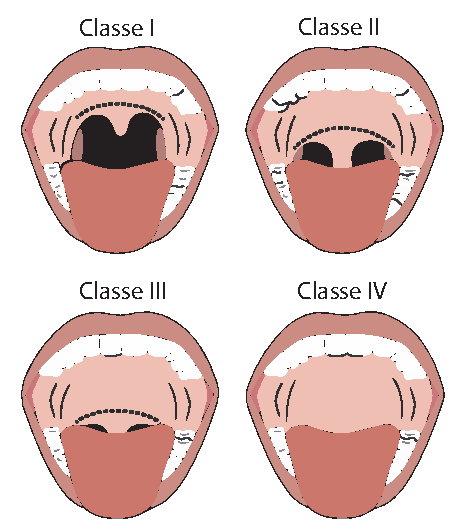
\includegraphics[width=0.5\textwidth]{Figure/mallampatpdf.pdf}
    \caption{Classificazione di Mallampati, adattata da \cite{Vargo2012}.}
    \label{fig:mallampati}
\end{figure}



\chapter{I farmaci}

Al fine di garantire un'ottima riuscita della procedura ed evitare nel bambino il ricordo di un'esperienza spiacevole e talora traumatica, ad oggi si può ricorrere sia ad interventi farmacologici di analgosedazione che ad interventi non farmacologici. Quest'ultimi possono essere utilizzati come metodo complementare o esclusivo, con innumerevoli benefici: dal ridurre l'agitazione preprocedurale e permettere una miglior transizione alla fase di sedazione, al contenere le dosi di farmaco utilizzate nel corso della procedura finanche, in alcuni casi, al prevenire del tutto il ricorso alla sedazione \cite{Uptodate}. Si tratta di approcci cognitivi e comportamentali che racchiudono tecniche di distrazione, rilassamento, desensibilizzazione e rinforzo positivo; risulta inoltre fondamentale, al fine di abbassare i livelli di ansia, instaurare una relazione di fiducia con i genitori e il bambino e definire un'adeguata strategia comunicativa, che adotti un linguaggio adeguato all'età o eventualmente introduca il gioco come strumento per prendere confidenza con le attrezzature mediche e le varie fasi della procedura. Tuttavia la sedazione farmacologica rimane la principale risorsa per agevolare le procedure più invasive. 

La scelta dell'agente farmacologico incide fortemente sulla qualità del risveglio post procedurale e va basata su diversi fattori. Premesso che il farmaco o la combinazione di farmaci selezionati deve indurre sedazione e analgesia adeguate a consentire il completamento della procedura con successo, mantenendo i riflessi protettivi delle vie aeree e l'autonomia cardiorespiratoria \cite{Krauss2006}, nel processo di decisione è importante valutare anche il livello di profondità della sedazione desiderato, conseguenza a sua volta del grado di analgesia richiesto dalla procedura. Infatti, talvolta è sufficiente solamente l'ansiolisi, altre volte è necessaria una più estesa analgesia, in altre occasioni invece lo scopo è quello di mantenere il paziente immobile, senza quindi bisogno di trattare il dolore. Altri elementi che guidano nella scelta del farmaco sono la familiarità nell'utilizzo da parte del sedatore e le caratteristiche individuali del paziente (età, comorbidità, allergie, grado di collaborazione, {\color{orange} ore di digiuno (?)}), che possono controindicare alcuni agenti farmacologici \cite{Uptodate}.
Infine, sono rilevanti alcune caratteristiche farmacocinetiche: sono infatti preferenziali farmaci con molteplici vie di somministrazione, induzione rapida e breve emivita, tale da concedere un celere recupero con assenti o minimi effetti collaterali.

Di seguito verranno dunque analizzate e confrontate le proprietà, i dosaggi, le indicazioni e gli effetti collaterali dei farmaci più comunemente utilizzati al di fuori della sala operatoria. 

\section{Propofol}

Il propofol è un sedativo ipnotico, non analgesico, il cui meccanismo d'azione a livello del sistema nervoso centrale non è del tutto noto, anche se ne è stata studiata l'interazione con il recettore A dell'acido $\gamma$-amminobutirrico (GABA) \cite{Propofol2015}.

\subsection*{Farmacodinamica}

Il legame tra le molecole di propofol e il recettore ionotropo GABA-A è responsabile degli effetti centrali del farmaco. Questo recettore è infatti un canale per il cloro presente a livello postsinaptico di molti neuroni. Una volta riconosciuto il ligando, si verifica un aumento del flusso degli ioni cloro attraverso la membrana, determinando iperpolarizzazione del neurone e {\color{orange}{refrattarietà}} agli stimoli esterni \cite{Propofol2015}.

\subsection*{Farmacocinetica}

Uno dei motivi per cui il propofol è ampiamente utilizzato riguarda proprio le sue vantaggiose caratteristiche farmacocinetiche: ha infatti un esordio d'azione estremamente rapido (30-45 secondi) ed un altrettanto rapido risveglio (5-15 minuti dopo singolo bolo, più lento in caso di infusione continua o boli multipli) \cite{Simeupsedazione, Uptodatepharmacology}. Si tratta di una molecola liposolubile, che supera la barriera ematoencefalica, macroscopicamente il propofol assume un aspetto lattescente e può essere somministrato solo per via endovenosa. Nel momento dell'iniezione può causare bruciore locale, che può essere prevenuto utilizzando una vena di calibro maggiore o diluendo a metà il propofol con soluzione fisiologica (5 mg/mL) \cite{Simeupsedazione}. 

\subsection*{Posologia}

Viene somministrato con un dosaggio di 1-2 mg/kg come bolo iniziale d'induzione, seguito da successivi boli multipli da 0.5 a 1 mg/kg ogni 2-3 minuti. Per le procedure più lunghe può anche essere utilizzato in infusione continua.
La dose massima è di 10 mg/kg totali per procedura \cite{Simeupsedazione}.

\subsection*{L'associazione con la ketamina}

Se la procedura è dolorosa il propofol può essere dato in combinazione con la ketamina, che oltre ad avere un'importante azione analgesica controbilancia gli effetti ipotensivo e bradicardizzante del propofol. Esistono in commercio delle formulazioni chiamate \emph{ketofol} con diversi rapporti di ketamina e propofol, tra i vantaggi risalta anche una minor incidenza di vomito e agitazione al risveglio, poiché l'effetto combinato permette di risparmiare ketamina \cite{Simeupsedazione}.

\subsection*{Effetti collaterali}

I principali effetti collaterali del propofol sono rappresentati dalla depressione respiratoria e dalla conseguente apnea, che dipendono dal dosaggio, dalla velocità di somministrazione e dalla risposta soggettiva del paziente. Inoltre, il propofol può determinare ipotensione e più raramente bradicardia \cite{propofolsafety2010}.
Un altro temibile quanto raro effetto avverso è costituito dalla \emph{sindrome da infusione di propofol}, potenzialmente fatale e descritta sia negli adulti che nei bambini \cite{Propofolinfusionsyndrome2019}. Si tratta di un insieme di segni e sintomi che si verifica in pazienti critici, che ricevono propofol in infusione a dosaggi elevati (>5 mg/kg/h) o per un periodo prolungato (>48h) ed è caratterizzata dalla presenza di una o più delle seguenti alterazioni, non spiegabili altrimenti: acidosi metabolica, rabdomiolisi, variazioni elettrocardiografiche associate o meno ad AKI, iperkaliemia, dislipidemia, scompenso cardiaco, febbre, elevazione degli enzimi epatici o del lattato. 

\section{Ketamina}

\lipsum[2]

\section{Midazolam}

\lipsum[3]

\section{Dexmedetomidina}

\lipsum[4]

\section{Protossido di azoto}

\lipsum[5]
 
\chapter{Analisi statistica: codici matlab}

\section{Raccolta e pulizia dei dati}
\label{code:wrangling}
\lstinputlisting[]{Dati/wrangler.m}

\section{Percezione globale dei quattro farmaci}
\label{code:quality-global}
\lstinputlisting[]{Dati/qualita.m}

\section{Esperienza sul campo e frequenza operativa}
\label{code:seniority-vs-experience}
\lstinputlisting[]{Dati/frequenza.m}

\section{Analisi stratificata su anni di esperienza e frequenza operativa}
\label{code:quality-strati}
\lstinputlisting[]{Dati/stratifica.m}

\section{Diversificazione degli effetti collaterali}
\label{code:adverse-effects-incidence}
\lstinputlisting[]{Dati/avversi.m}

\section{Come gli effetti collaterali incidono sulla percezione del farmaco}
\label{code:adverse-effects-perception}
\lstinputlisting[]{Dati/pericolosita.m}

\section{Frequenza d'impiego di tecniche di distrazione}
\label{code:misdirection-techniques}
\lstinputlisting[]{Dati/distrazione.m}

\section{Frequenza d'impiego di farmaci \emph{rescue}}
\label{code:rescue}
\lstinputlisting[]{Dati/rescue.m}

\section{Grado di sicurezza globalmente percepito}
\label{code:safety}
\lstinputlisting[]{Dati/sicurezza.m}

\section{Fattori preponderanti nella percezione globale}
\label{code:satisfaction}
\lstinputlisting[]{Dati/soddisfazione.m}

\newpage

\section{Sotto-routine utilizzate nei codici}
\label{code:subroutines}
\lstinputlisting[]{Dati/palette.m}
\lstinputlisting[]{Dati/boxplot.m}
\lstinputlisting[]{Dati/save_fig.m}
\end{appendices}

%>RINGRAZIAMENTI
\setcounter{secnumdepth}{-1}
\chapter{Ringraziamenti}
%\addtocentrydefault{chapter}{}{Ringraziamenti}
%\addcontentsline{toc}{chapter}{Ringraziamenti}

Questo spazio lo dedico alle persone che, con il loro supporto, mi hanno aiutato in questo lungo quanto arricchente percorso universitario. 

\bigskip \noindent
Ringrazio innanzitutto il mio relatore, prof. Barbi, per l'impareggiabile disponibilità e per avermi trasmesso nozioni che non si possono apprendere dai libri.

\bigskip \noindent
Un ringraziamento speciale alla mia correlatrice, dott.ssa Martina D'Agostin, che ha saputo guidarmi con pazienza ed entusiasmo in ogni step della realizzazione di quest'elaborato. %e lasciando spazio alle mie idee. 

\bigskip \noindent
Al mio ragazzo Gabriele: grazie per esserci sempre stato e per aver creduto in me incondizionatamente, anche nei momenti in cui vedevo questo obiettivo gigante e irraggiungibile. Grazie per avermi insegnato a trasformare la paura in coraggio e per avermi spinta ad essere più sicura, consapevole e fiduciosa in me stessa: continuerò comunque a chiederti di leggermi le mail prima di inviarle. Ti ringrazio, inoltre, per aver condiviso con me le tue nozioni di programmazione ed avermi pazientemente aiutato con i contenuti grafici e l'analisi statistica. Senza di te e la tua inarrestabile pignolaggine questo lavoro di tesi non sarebbe altrettanto ben fatto.

%Grazie per avermi insegnato ad avere coraggio, nonostante la paura. Grazie per essere ed essere stato in questi anni il mio compagno di avventure  e il mio migliore amico, semplicemente la mia persona e grazie per avermi dato l'opportunità di arricchire il mio bagaglio di conoscenze, idee, opinioni, grazie alle nostre discussioni e ai nostri confronti sui temi più svariati. Grazie perché se sono orgogliosa della persona che sono oggi è anche merito tuo.  Infine, 

\bigskip \noindent
Ringrazio i miei genitori per avermi sempre sostenuto, supportato e per avermi permesso di portare a termine gli studi universitari, aiutandomi ad affrontare i momenti più difficili. 

\bigskip \noindent
Ringrazio mia sorella Viola per avermi mostrato che dalla costanza e dall'impegno nascono i migliori risultati ma soprattutto per i post-it motivazionali. Non li dimenticherò. 

\bigskip \noindent
Grazie alla mia nonnina Ester, che ha pazientemente atteso questo traguardo e che è quasi più emozionata di me nel vedermi, finalmente, conquistarlo.

\bigskip \noindent
Un grazie sincero ai miei amici Giulia N., Giulia O. e Andrea, che sono sempre stati pronti ad ascoltarmi ed aiutarmi attivamente durante tutte le difficoltà incontrate in questi ultimi mesi. 

\bigskip \noindent
Grazie alle mie coinquiline Fra e Sere che hanno condiviso con me le gioie e i topi di questo percorso, vi voglio bene e vi avrò sempre nel cuore. 

\bigskip \noindent
Grazie ad Ariettis per aver reso spumeggiante e vivernosa quest'esperienza e grazie per tutte le volte che mi hai spinta a buttarmi: senza i tuoi incitamenti ora avrei fatto la metà degli esami.

\bigskip \noindent
Grazie a Jimmy per essere stato la mia colonna sonora del liceo ed essere rimasto il mio compagno di banco, anche se a 170km di distanza. Grazie per aver ascoltato ogni mio singolo audio di 8 minuti e grazie per essere stato il primo ad avermi fatta sentire un "medico": spero che la qualità miei consigli medichesi migliorerà sempre di più. 

\bigskip\noindent
Infine, grazie a tutti i miei amici vicini e lontani, ai miei compagni di università e a tutti quelli che hanno incrociato la loro vita con la mia lasciandomi un insegnamento, una risata, un'emozione: grazie per essere stati parte di questi otto lunghi, intensi ed entusiasmanti anni.

\bigskip\noindent
Quasi dimenticavo: grazie geco per la tua vicinanza poco prima del mio ultimo esame, sei stato un terrificante portafortuna. 

\bigskip\noindent
Grazie, infine --questa volta per davvero-- al mio anaffettivo quanto esuberante gatto Joule per essere stato mio fedele compagno di studi e per i sorrisi che mi hai strappato tutte le volte che distoglievo lo sguardo dai libri e ti trovavo comodamente seduto, come il più ordinario degli umani. Anche se non sai leggere, grazie per avermi rubato il cuore e per avermi insegnato, con la tua superiorità felina, di amare sempre prima se stessi.  

%>BIBLIOGRAFIA
\printbibliography[heading=bibintoc,title={Bibliografia}]

\end{document}





